\subsection{Análise Relacionada à Primeira Questão de Pesquisa}

A primeira questão de pesquisa busca verificar a facilidade de compreender (ou adotar) a abordagem proposta neste trabalho de dissertação. Para isso, foi aplicada uma pesquisa qualitativa cujos dados foram coletados por meio de um questionário.

Inicialmente, buscou-se saber a experiência dos participantes em Engenharia de Software e em projetos envolvendo \acrshort{SOA}. Observando a Figura~\ref{fig:experiencia_sw}, verificou-se que os participantes tem boa experiência com Engenharia de Software: apenas 20\% tem 1 ano de experiência, os outros 20\% tem entre 2 à 5 anos, 30\% tem entre 5 à 10 anos e os demais 30\% tem mais de 10 anos de experiência. Quando comparado com a experiência em projetos orientados a serviços, 30\% dos participantes alegaram não ter nenhuma experiência, como mostra a Figura~\ref{fig:experiencia_soa}. Além disso, metade dos participantes disseram ter trabalhado em 1 projeto, possivelmente o próprio \acrshort{SAE} da UnB. Os demais participantes trabalharam em 2 ou mais projetos. Posteriormente, quando questionado se a empresa onde trabalham pretendem desenvolver projetos em \acrshort{SOA} nos próximos 6 meses, 90\% indicaram que sim.

% Figura que mostra a experiência em Engenharia de Software
%======================================================================================

\begin{figure}[htb]
\centering
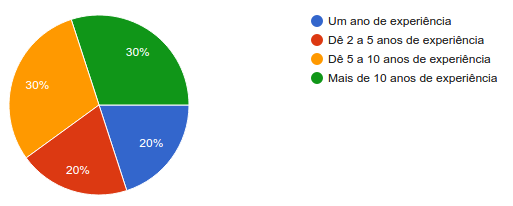
\includegraphics[scale=0.72]{/img/avaliacao/QP1/experiencia_sw.png}
\caption{Experiência dos participantes em Engenharia de Software.}
\label{fig:experiencia_sw}
\end{figure}
\FloatBarrier


Em seguida, foi solicitado que os participantes descrevessem a sua experiência com a abordagem \acrshort{SOA} proposta neste trabalho de dissertação, em termos de compreensão e facilidade de uso. De acordo com as respostas obtidas, a abordagem foi considerada relativamente simples. Por exemplo, o participante 1 considerou a experiência satisfatória e de grande importância para difusão do conhecimento sobre \acrshort{SOA} que tem vindo a ser cada vez mais adotada nas organizações. Os participantes 2 e 3 disseram ter experimentado \acrshort{SOA} pela primeira vez. O participante 8 ressaltou ter sido o primeiro contato com o estilo arquitetural RESTful e que já conseguiria divulgar e aplicar os conhecimentos adquiridos.


% Figura que mostra a experiência em SOA
%======================================================================================

\begin{figure}[htb]
\centering
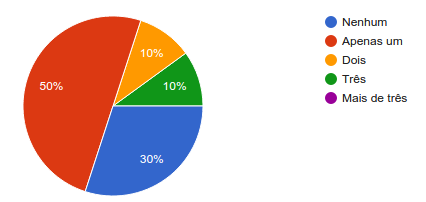
\includegraphics[scale=0.72]{/img/avaliacao/QP1/experiencia_soa.png}
\caption{Experiência dos participantes em \acrshort{SOA}.}
\label{fig:experiencia_soa}
\end{figure}
\FloatBarrier

Os participantes tiveram que informar também as atividades por ordem de relevância consideradas mais complexas na modernização do \acrshort{SAE}. Nesse caso, 50\% dos participantes escolheram a definição da Direção Estratégica do projeto, seguindo de 30\% para a Especificação do Modelo de Domínio do Negócio, como ilustra a Figura~\ref{fig:primeira_atividade_complexa}. Os demais escolheram outras opções ligadas a atividade Analisar e Projetar os Serviços, conforme o processo da abordagem proposta. 

Uma das razões que se supõem, para a definição da Direção Estratégica ser considerada a atividade mais complexa do estudo de caso, está relacionada ao alinhamento dos \textit{stakeholders} (principalmente os gestores do CPD/UnB) para decidirem o sistema a ser modernizado e a estratégia de modernização a ser utilizada. Ou seja, segundo a nomenclatura proposta por~\cite{S3_Bisbal:1999}, seria através de uma migração ou uma substituição? 

Como foi visto no \acrshort{MS} realizado no Capítulo~\ref{mapeamento}, a migração visa mover o sistema legado para um ambiente mais flexível, mantendo os dados e funcionalidades originais enquanto que a substituição busca desenvolver um sistema completamente novo. Nesse caso, os participantes decidiram modernizar o sistema por meio de uma substituição, já que seria necessário rever os requisitos com os usuários e possivelmente reestruturar o esquema do banco de dados do \acrshort{SAE}. Entende-se que tal decisão foi possível porque o \acrshort{SAE} é um sistema relativamente pequeno e com pouco impacto nos demais sistemas da UnB, de acordo com os analistas do CPD. Até porque, na análise da QP2 do \acrshort{MS} para identificar quais processos, técnicas ou ferramentas têm sido sugeridos na literatura para suportar as atividades de modernização dos sistemas legados, apenas 1 projeto sugere tal abordagem, em grande parte, por causa dos riscos envolvidos com essa estratégia de modernização~\cite{S3_Bisbal:1999, Comella-DordaASurvey2000, Salvatierra:2013}. 

Prosseguindo com a análise, verificou-se que o Primeiro Contato e o Entendimento Inicial do sistema escolhido não foi considerada uma atividade complexa. Em contrapartida, 30\% dos participantes avaliaram a Especificação do Modelo de Domínio do Negócio do sistema \acrshort{SAE} como muito difícil, face as inúmeras dúvidas sobre como identificar, modelar e organizar os serviços através de uma arquitetura de software adequada a \acrshort{SOA}. 

No que concerne ao Primeiro Contato e Entendimento Inicial, os participantes do estudo de caso investiram um tempo considerável para obter uma compreensão adequada do sistema \acrshort{SAE}. Contudo, observa-se que muitas vezes o CPD/UnB não despende tanto esforço para compreender um sistema existente como deveria e algumas técnicas que poderiam ser úteis, como a análise estática, não são utilizadas. 

Algumas outras atividades também foram consideradas notoriamente difíceis 
pelos participantes do estudo de caso, a exemplo da reestruturação do esquema do banco de dados do \acrshort{SAE} (veja a Figura~\ref{fig:classificacao_reestruturacao_bd}) e a identificação dos serviços que foi necessário fazer na atividade Analisar e Projetar Serviços. Por curiosidade, fez-se um questionamento para saber que técnica auxiliou mais na identificação dos serviços, sendo que 50\% dos participantes indicaram a geração do catálogo de serviços (analisando a estrutura de tabelas do banco de dados e seus relacionamentos) ajudou mais que a própria inspeção das telas (30\%) e a análise estática do código fonte (10\%) do \acrshort{SAE}. Acredita-se que seja porque isso permitiu focar na interface dos serviços. Além do mais, os participantes podiam simular a execução dos serviços com ferramentas \acrshort{REST} disponíveis\footnote{A ferramenta \acrshort{REST} Advanced Client foi uma das ferramentas utilizadas para executar os serviços publicados no barramento.} mesmo sem os serviços estarem implementados, contribuindo tanto para uma melhor compreensão dos serviços oferecidos como também para auxiliar na obtenção de um design de \acrshort{API} melhor projetada. A Figura~\ref{fig:melhor_tecnica_compreensao} ilustra esse resultado. 


Para finalizar a resposta desta questão, os maiores desafios identificados foram a Direção Estratégica e a Especificação do Modelo de Domínio do Negócio, duas atividades consideradas gerenciais e de análise. Entende-se que o direcionamento estratégico seja um desafio comum em qualquer projeto de modernização de software, não precisando ser utilizado a abordagem proposta. A especificação do modelo de domínio do negócio também é uma atividade bastante complexa independente de se utilizar SOA, sendo que, nesse projeto de modernização, pelo fato do sistema legado \acrshort{SAE} ser procedimental, dificultou enormemente a identificação e a modelagem dos serviços. No que compete ao desenvolvimento dos serviços, a arquitetura concebida permitiu um fácil desenvolvimento pelo que se observou durante o estudo de caso e a partir das respostas do questionário, sendo possivelmente, um indicador de boa manutenibilidade. Esse fator será analisado na próxima questão.






\begin{figure}[htb]
\centering
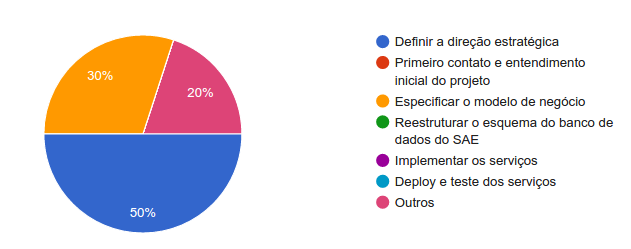
\includegraphics[scale=0.72]{/img/avaliacao/QP1/primeira_atividade_complexa.png}
\caption{Atividades mais complexa na modernização do \acrshort{SAE}.}
\label{fig:primeira_atividade_complexa}
\end{figure}



\begin{figure}[htb]
\centering
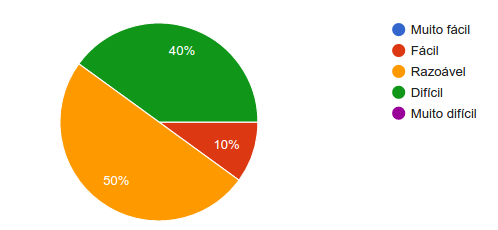
\includegraphics[scale=0.72]{/img/avaliacao/QP1/classificacao_reestruturacao_bd.png}
\caption{Dificuldade para reestruturar o esquema do banco de dados do \acrshort{SAE}.}
\label{fig:classificacao_reestruturacao_bd}
\end{figure}



\begin{figure}[htb]
\centering
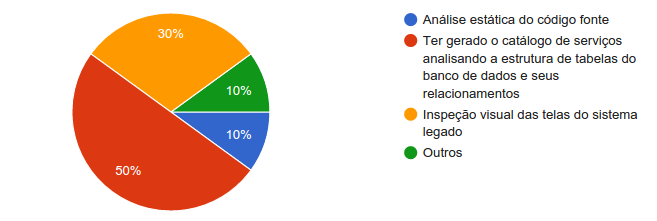
\includegraphics[scale=0.72]{/img/avaliacao/QP1/melhor_tecnica_compreensao.png}
\caption{Qual a técnica que mais contribuiu na compreensão do \acrshort{SAE}.}
\label{fig:melhor_tecnica_compreensao}
\end{figure}




